%% This is an example first chapter.  You should put chapter/appendix that you
%% write into a separate file, and add a line \include{yourfilename} to
%% main.tex, where `yourfilename.tex' is the name of the chapter/appendix file.
%% You can process specific files by typing their names in at the 
%% \files=
%% prompt when you run the file main.tex through LaTeX.

\chapter{ChromoZoom v2: dynamic, online visualization of genomes and next-generation sequencing data}

\begin{marginfigure}[1cm]
  
\includegraphics[width=\textwidth]{chap3/chromozoom-gray}
  The genome browser that lets you fly.
\end{marginfigure}

\begin{quote}
\emph{Although new sequencing technologies enable the automatic assembly of complete genomes from long reads along with copious layers of functional data, sharing and collaborating on these datasets remains difficult with current software. Genome browsers are the standard approach for interactively exploring these data and can also facilitate collaboration if they are accessible via the web. The first version of ChromoZoom was written in 2012 as a fast, fluid web interface for genome browsing, although the design centered around scraping data for three reference genomes. With the present pace of \emph{de novo} assembly and growth in the number of reference genomes, this strategy requires some rethinking. Here, we present a re-engineered version of ChromoZoom that can dynamically load custom genome assemblies and related data and also adds many new features that support pathogen surveillance activities at Mount Sinai.}
\end{quote}

\section{Introduction}

\newthought{Genome browsers are indispensible} tools for modern experimental and computational biology. The size of typical genomic data (anywhere from tens of thousands of nucleotides for viruses into the billions for humans) prevents static plots from simultaneously capturing its scale and detail in a reasonable amount of space. Therefore, genome browsers are tasked with laying out the data in a way that is both interpretable and interactively navigable. Most designs use a movable viewing region and map the contigs (in a completed assembly, the largest of which are the organism's chromosomes) to one axis of the coordinate system, usually a horizontal axis, while stacking the datasets onto the other axis. These other data can include range features such as genes and coding regions, continuous quantitative data like read depth and methylation levels, and mappings of other sequences, such as a different genome or the reads from a sequencing experiment. Many other datatypes exist and continue to be invented, but these are the basic shapes of data that genome browsers are expected to handle.

Current genome browsers fall into three major categories, each with their own advantages and disadvantages. In fetching and drawing large amounts of heterogenous data, \emph{desktop-based browsers} like IGV,\autocite{Thorvaldsdottir2013} IGB,\autocite{Freese2016} and SmrtView\footnote{\url{https://github.com/PacificBiosciences/DevNet/wiki/SMRT-View}} have retained an advantage in being fastest during typical navigation operations, particularly when the data is being read from the user's local hard disk. All of the aforementioned desktop applications, however, use Java; this incurs the penalty of installing a Java VM alongside the browser, and precludes their use on many mobile devices. Because of the need to the download software, these applications are not well-equipped for the rapid sharing of an active browsing session with a colleague, as website users are accustomed to doing by sending a URL or using ``share'' buttons. Nevertheless, they remain very popular for browsing of large alignments from routine next-generation sequencing (NGS) experiments on humans and model organisms, since the size (and potential confidentiality) of these data often prevent them from being sent over the internet to web-based genome browsers. 

The first generation of web-based genome browsers like UCSC,\autocite{Dreszer2011} GBrowse,\autocite{Stein2002} Ensembl,\autocite{Stalker2004} and the NCBI Map Viewer\autocite{Wheeler2003} continue to retain the advantage of instant access from any web browser and the simplicity of sharing a particular view of the genome by linking to it. Since they were some of the first genome browsers to gain widespread use by wet lab biologists, and offered centralized repositories of valuable data during key moments of the dawn of human genomics, they still tend to exhibit the widest array of well-curated data. UCSC's browser is well known for having being the first to provide rapid, interactive access to early products of the Human Genome Project,\autocite{Kent2002} and remains prominent in human genomics for having thousands of widely-used tracks covering everything from tissue-specific expression and evolutionary conservation to clinically significant variants. However, since these software projects were built before modern web technologies like Asynchronous Javascript (AJAX) and HTML5, the server must draw each user's data as an image that is sent to their browser, and the software's interactivity is therefore constrained compared to newer web applications. Unlike, e.g., Google Maps, none of these browsers allow the user to smoothly scroll, zoom, or ``throw'' the viewport (also called inertial scrolling), and they cannot draw new data without interrupting the user's movements. This latency makes it frustrating to gain an intuitive feel for distances or zoom levels and clashes with the experience users expect from the way scrolling\footnote{And pinching, since the release of the iPhone. Both operations on modern smartphones take pains to stay at a buttery smooth 60fps, even if rendering quality has to be temporarily downgraded.} works on most other apps and websites.

Around 2009, a new generation of web-based genome browsers that embraced AJAX\autocite{Paulson2005} and employed JavaScript to dynamically draw data on the client-side emerged. Of these, projects that have stayed active include JBrowse,\autocite{Buels2016} Dalliance,\autocite{Down2011} and Anno-J.\footnote{\url{http://www.annoj.org}} Among their advantages were a level of interactivity that approached the look and feel of the desktop-based browsers, without a need to download and install any software. Additionally, in some cases, views of the data could be shared as in the older web-based browsers. However, the new browsers have become largely divorced from the extent of track curation that is integral to older web-based genome browsers, providing only barebones demo sites to try out the software on a small number of tracks. Including the most recent entrants in this category, pileup.js\autocite{Vanderkam2016} and igv.js,\footnote{\url{https://github.com/igvteam/igv.js}} all of the next-generation genome browsers are primarily provided as source code libraries, which expect the users to install the code to their own web server and marry it to data via configuration or the embedding of components into a larger website. Obviously, this reduces the accessibility of the software to teams with a web developer and a webserver.

There still is no genome browser that hits all the high marks of Google Maps in providing a (1) universally accessible, (2) richly interactive, and (3) easily sharable visualization of large, multilayered datasets. Without requiring any additional software, Google Maps even allows users to add custom data that is plotted on top of a map, and then share it via URL or embed it into another site.\footnote{An example of a running route in New York City: \url{https://goo.gl/GoHxx8}} Although Dalliance and JBrowse do offer some UI panels for layering user-provided data onto the server-provided tracks, they don't offer any sharing capabilities for these ``mashup'' views. In fact, none of the newer generation of web-based genome browsers emphasize this use case, suggesting that custom data should be configured by the server administrator. Finally, despite the increasing production of new genome layouts (or reference assemblies) as \emph{de novo} assembly of NGS data becomes commonplace, none of the new generation of web-based genome browsers allow a user to dynamically load custom genomes (with or without annotations) via their UI. Therefore, there are still avenues for improving web-based genome browsers to reach the level of the user experience that Google Maps had standardized by 2004.\autocite{Vincent2007}

\section{Implementation}

The first version of ChromoZoom,\autocite{Pak2013a} released in 2012 at \url{http://chromozoom.org/}, attempted to achieve the three previously enumerated design goals, but targeted a small set of reference genomes in UCSC's database: GRCh37/hg19 (Human, Feb. 2009), NCBI36/hg18 (Human, Mar. 2006), and sacCer3 (Baker's yeast, Apr. 2011). At the time, we pursued a strategy of scraping UCSC's rendered images for these genome tracks at multiple zoom levels and serving them as tiles, similar to the approach of the first version of Google Maps.\footnote{See \textcite{Skinner2009}. Today, Google Maps renders all data using \href{https://developer.mozilla.org/en-US/docs/Web/API/WebGL_API}{WebGL} when available, which allows for GPU acceleration in the browser and higher framerates.} Our approach ran into several roadblocks over time. Firstly, due to space constraints, it was impossible to scrape tiles for all of the thousands of tracks that UCSC hosts, so we had to focus only a commonly used subset for the two human assemblies. Secondly, since it was so computationally expensive to render all the tiles for a new genome, there was no expectation that the user could ever load a previously unseen genome assembly (or request that it be loaded) from the client side. Finally, the cost of re-rendering tiles made it difficult for us to keep tracks up to date with UCSC's data, even after we created a complete local mirror of the UCSC genome browser. Although ChromoZoom did allow for user-provided custom data to be drawn alongside the tiled images using client-side JavaScript and \texttt{<canvas>} elements, we expected that server-hosted tracks would remain more popular.

As demand for different genome assemblies and more varieties of custom data grew, we realized that our server-side tile scraping strategy would be untenable in the long run. Particularly in the context of pathogen surveillance and microbiology, where the number of completed reference genomes for certain species is already in the hundreds,\footnote{As of April 2017, there are 154 complete \emph{Staphyloccocus aureus} genomes on NCBI Genome: \url{https://www.ncbi.nlm.nih.gov/genome/genomes/154}} there was a severe need for a web-based genome browser that could dynamically load a custom genome assembly with associated sequence, alignment, and annotation files and render them all on the client side. Although desktop-based genome browsers (particularly IGB) are capable of opening custom assemblies, their visualizations are not easily shared amongst a diverse team of wet lab biologists, bioinformaticians, and clinicians.

Therefore, we re-engineered ChromoZoom v2 to support a new strategy of displaying every genome entirely via the use of \texttt{<canvas>} and SVG with client-side parsing and display of all contig layout, track annotation, and sequence data. The efficient requesting and download of track data that overlaps the user's current viewport is enabled by the use of bigBed and bigWig formats,\autocite{Kent2010} which are compressed binary files that exceed the storage efficiency of our previous tiled-image approach. To test whether this new strategy scales, we scraped all active genomes from UCSC using a custom pipeline, written in Python, that converts data from UCSC's MySQL dumps into the bigBed and bigBed formats, and we now provide all UCSC genome data via this mechanism, not as tiled images.

ChromoZoom is still implemented as a single-page web application that heavily relies on JavaScript, particularly the jQuery UI library, and it is compiled into a single bundle using \texttt{browserify}.\footnote{\texttt{browserify} is \texttt{nodejs} package that can combine multiple JavaScript source files, including \texttt{node} modules, into a single bundle. See: \url{http://browserify.org/}} All genomic data is fetched via AJAX and a thin layer of PHP that interfaces with libraries and utilities for each data format, possibly retrieving the data from a distant server.

For client-side performance, we continue to use tiled HTML5 elements that are rescaled and moved in accordance with user pan, zoom, and throw operations. We prerender into off-screen tiles to maintain a sense of location even when the viewport moves or zooms. For maximal performance when animating these elements during viewport movement, we use the GreenSock Animation Platform.\footnote{GreenSock uses CSS3 transforms to enable hardware acceleration where possible. See \url{https://greensock.com/}} To the greatest extent possible, fetching and parsing of track data and genome data occurs within Web Workers, which offload execution of JavaScript into processes that don't block the browser's main UI thread; this is a unique performance advantage of ChromoZoom over other next-gen genome browsers.\autocite{Buels2016,Down2011,Vanderkam2016} Although most rendering is done into rasterized \texttt{<canvas>} tiles for performance reasons, we fully support high-DPI (i.e., ``retina'') displays by always rendering at the native pixel resolution of the display device.

\subsection{Availability}

ChromoZoom's source code is available from github at \url{https://github.com/rothlab/chromozoom}. ChromoZoom v2 can be viewed online by nearly any modern web browser (Chrome, Safari, Firefox, or IE11+) at \url{http://chromozoom.org/}.

All code is available under an AGPLv3 license\footnote{Briefly, this means that you can use ChromoZoom code for derivative web applications, as long those web applications are also open source. See \url{https://www.gnu.org/licenses/agpl-3.0.en.html}} and is free for academic and personal (but not commercial) use. For those that want to develop using ChromoZoom code or deploy it locally (e.g., to view or serve data within a firewall), it can be installed to any Linux or macOS server with Apache web server, PHP 5.x, and a collection of executables from \texttt{samtools} and Jim Kent's utilities, both of which are freely downloadable.\footnote{See \url{http://www.htslib.org/download/} and \url{http://hgdownload.cse.ucsc.edu/admin/exe/}.}

\section{Results and Discussion}

\subsection{Data mirrored from UCSC}

183 genomes from UCSC were scraped for all track types compatible ith ChromoZoom v2, which includes bigWig, bigBed, BAM, tabix-compressed VCF,\autocite{Danecek2011,Li2011} wiggle, and BED, and formats convertible to compatible formats, which includes genePred, rmsk, PSL, GVF, and narrowPeak.\footnote{Descriptions of all formats can be found at \url{https://genome.ucsc.edu/FAQ/FAQformat.html}} This produced 8,702 converted bigBed files and 7,670 additional track entries that point directly to big* format files on UCSC's servers. Collectively, the scraped tracks consume 485 GB of disk space. Since UCSC's MySQL database contains information on the update time for each table, we can re-run this process on a weekly schedule and only re-download data for tracks that have been updated. We therefore can continually and efficiently keep our bigBed files synchronized with UCSC's database.

\subsection{Browsing a custom bacterial genome assembly}

Figure \ref{fig:bacterial_overall} provides an overview of the ChromoZoom v2 browser interface being used to visualize an assembled isolate of \emph{Staphyloccocus aureus} from The Mount Sinai Hospital.\footnote{The isolate was sequenced and assembled using the methods described in \autoref{chap:steno}.} The interface uses the top line to display navigational controls, while the genome selection menu is in the lower right. This menu displays ``Custom Genome'' because the genome layout was not provided by the browser, but was loaded from another source—specifically, an IGB Quickload Directory. Supported formats for custom genomes will be covered later in this article.

\begin{figure*}[htb]
  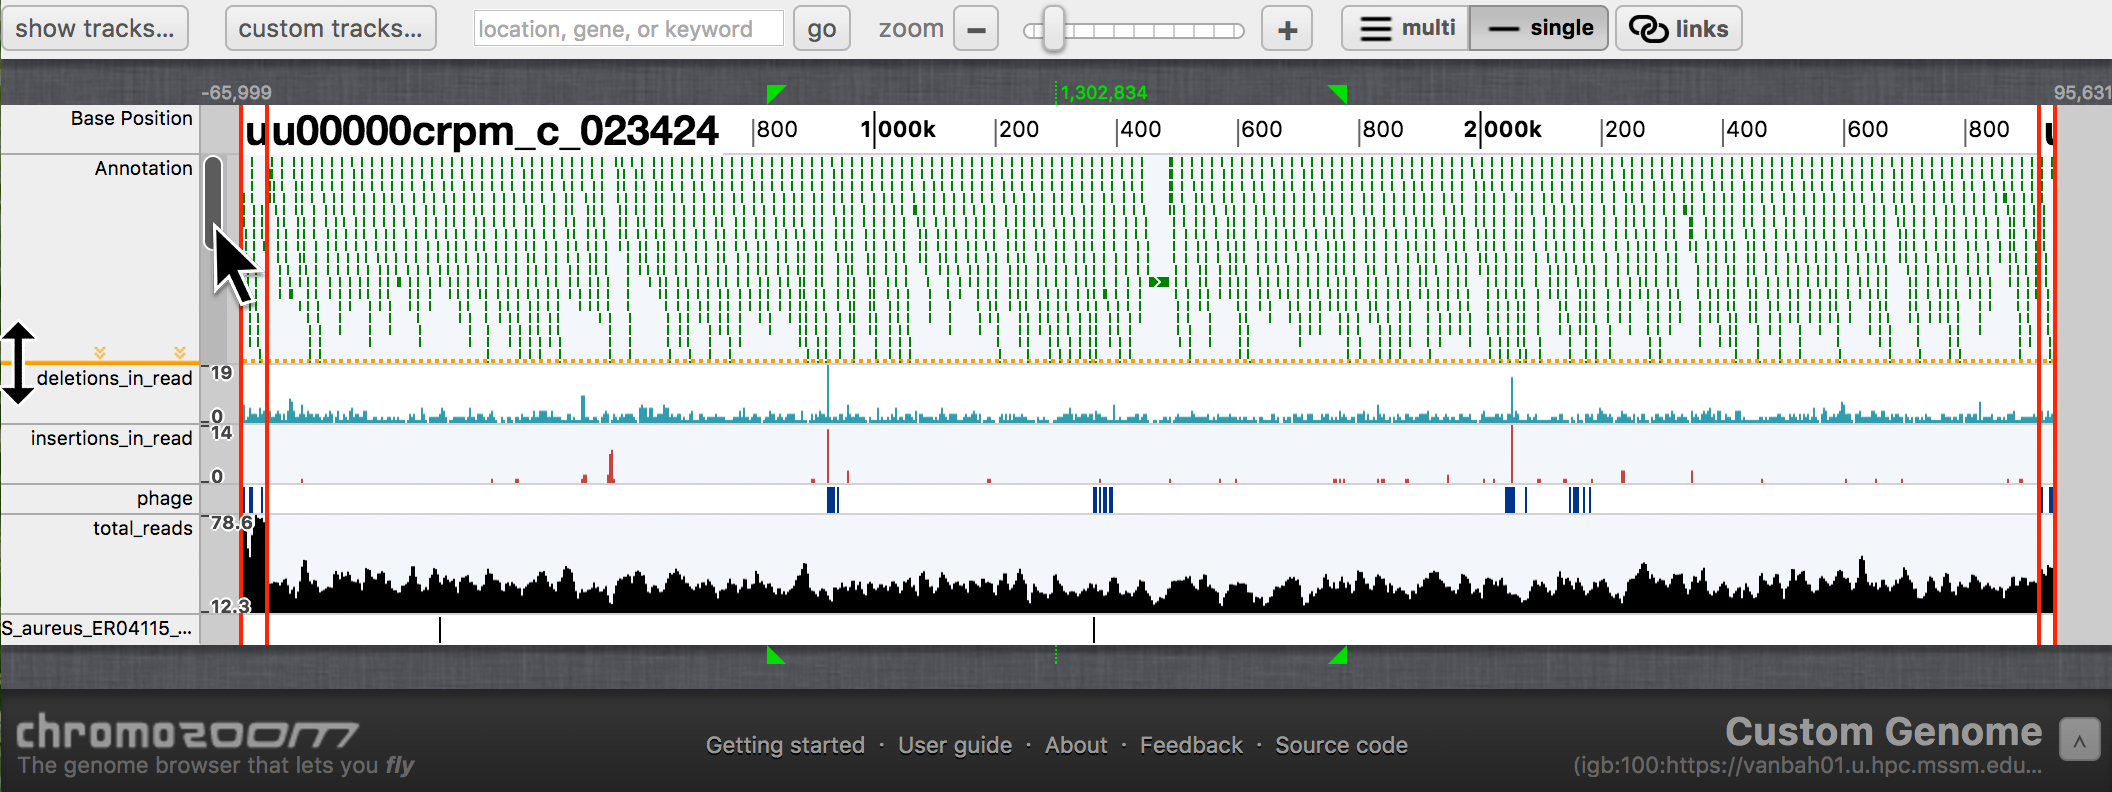
\includegraphics[width=\textwidth]{chap3/bacterial-ER04115}               
  \caption[Browsing a completed \emph{S. aureus} assembly with two plasmids]{Browsing a completed \emph{S. aureus} assembly with two plasmids (leftmost and rightmost small contigs).}
  \label{fig:bacterial_overall}
\end{figure*}

Data is placed front and center in the main area of the interface. The user can click, drag, and throw this area horizontally to move. A green ``tank reticle'' is visible in the center of the screen, which helps provide feedback during zooming operations with the mousewheel and highlights the coordinate that the user is zooming on. The display is at nearly the lowest zoom setting, so all three contigs are visible, and are separated by the bright red lines. The names of contigs are shown as the large labels in the ``Base Position'' track. Ticks in this track follow a minimalist format that avoids duplication of nonsignificant digits.\autocite{Krzywinski2013}

Six additional tracks are being displayed in this view, which are labeled along the left side of the tracks. The top track, in green, contains gene annotations by \texttt{prokka};\autocite{Seemann2014} this was supplied as a BED track. There are many such annotations in all contigs, and the orange dotted indicator below this track warns the user that some of the data is being clipped by the vertical space available. A scrollbar is available at the leftmost edge of the track to view the bottom edge of the track. 

The next two tracks in turquoise and red are bigWig tracks that count the number of deletions or insertions in reads, binned by based position. Two regions of globally maximal insertions and deletions are notable, which happen to correspond with features in the next track, which contains annotated phage regions.\footnote{This track was generated with \texttt{scripts/get\textunderscore repeats\textunderscore phage\textunderscore pai.py}, written by Mitchell Sullivan and incorporated into \href{https://github.com/powerpak/pathogendb-pipeline}{pathogendb-pipeline}.} These regions also appear to correlate with troughs in the read depth, which is plotted in the ``total\textunderscore reads'' track. The last track shows single nucleotide variants (SNVs) created from a comparison using \texttt{nucmer} against a closely related hospital strain. Since there are only 2 SNVs separating these strains, they are related enough to consider that transmission (either between the patients or from a common source) was very likely.

\begin{marginfigure}
  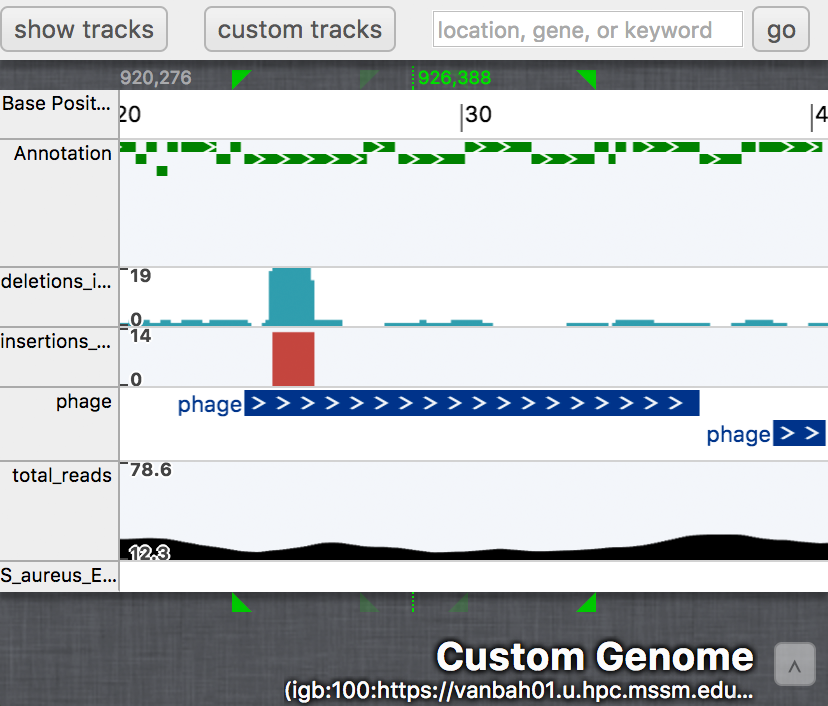
\includegraphics[width=\textwidth]{chap3/bacterial-phage}               
  \caption[A phage region corresponds to high insertion/deletion density.]{A phage region corresponds to high insertion/deletion density.}
  \label{fig:bacterial_phage}
\end{marginfigure}

A zoomed view of the leftmost phage region in the large chromosomal contig is shown in Figure \ref{fig:bacterial_phage}. This screenshot also highlights the responsiveness of the UI to resizing of the window: ChromoZoom is usable on displays as small as a smartphone screen. It is clear that the region with increased insertions and deletions is indeed in the middle of a phage region and a coding region annotated by \texttt{prokka}. An even closer look is shown in Figure \ref{fig:bacterial_phage_variability}, which adds an alignment track (in BAM format) of error-corrected reads created during the Hierarchical Genome Assembly Process.\sidecite[-1em]{Chin2013}
\begin{figure}
  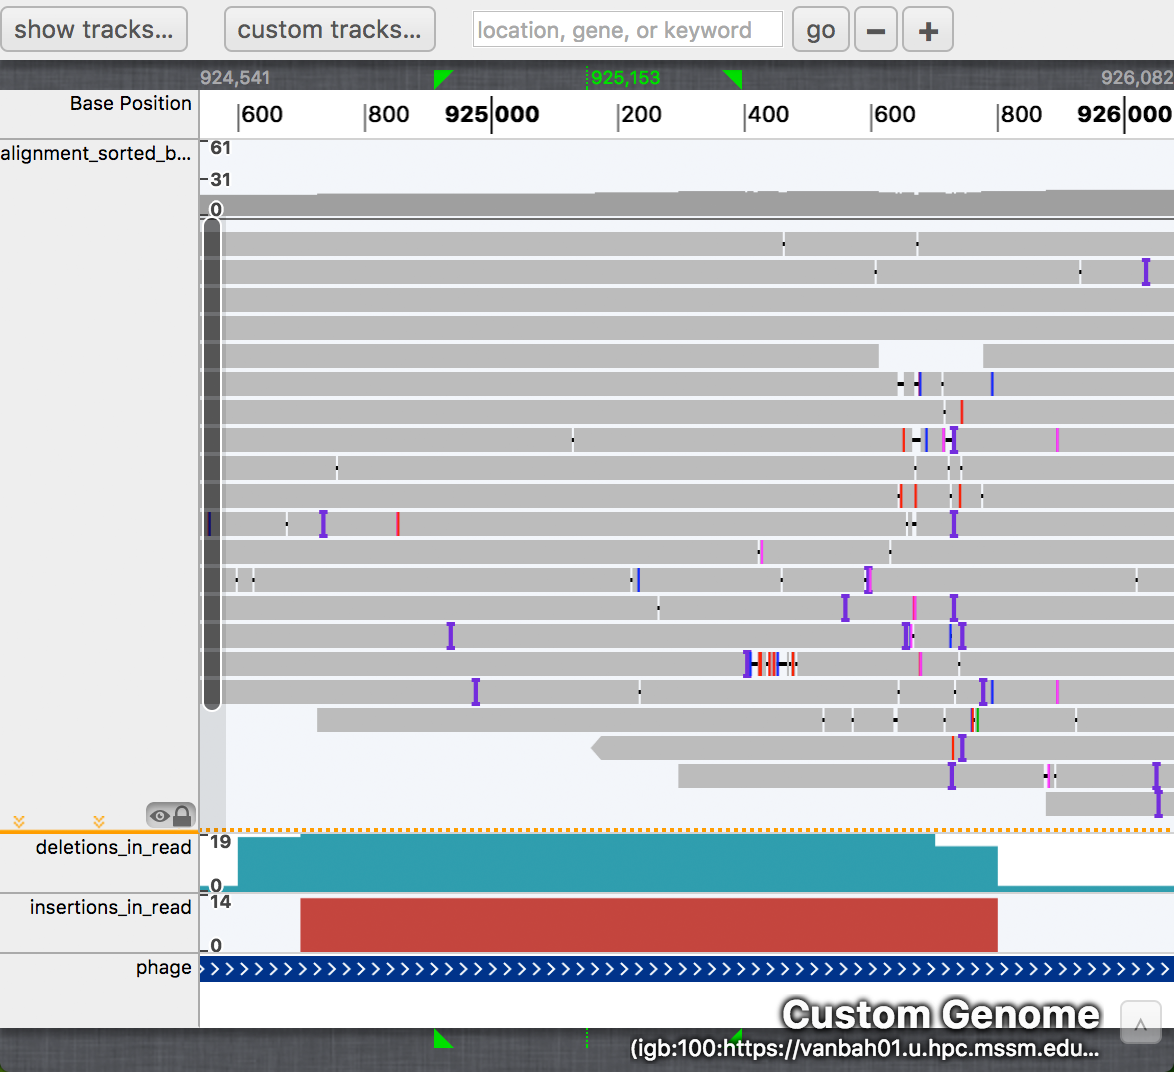
\includegraphics[width=\textwidth]{chap3/bacterial-phage-hypervariability}               
  \caption[Confirmation of a hypervariable region among phage genes]{Confirmation of a hypervariable region among phage genes. An alignment of error-corrected reads to the finished assembly has been added as the top track, using conventions for displaying BAM files that are similar to IGV. A coverage graph on the top of the track displays the depth of aligned reads, while the alignments themselves are displayed in a stack below, with notation symbols described in the main text. Judging from the totality of the evidence among all reads, the hypervariable region is approximately 200bp long and spans from 925,600 to 925,800.}
  \label{fig:bacterial_phage_variability}
\end{figure}
These alignments show how the error-corrected reads align to the final contigs created during assembly. The track uses display conventions similar to IGV:\autocite{Thorvaldsdottir2013} each aligned preassembled read is depicted as a gray block, with gaps relative to the reference shown as a horizontal black line, and insertions relative to the reference shown as the vertical purple I-bars. Single-base mismatches are depicted as colored vertical stripes in each read. From this view, it appears that an approximately 200bp region is particularly enriched for indels among the majority of the error-corrected reads, and therefore may represent a hypervariable region. Bacteriophages are known to contain genetic elements that generate diversity by site-directed, adenine-specific mutagenesis via reverse transcriptase-mediated exchange between two repeats in order to alter their tropism and possibly also to evade the human immune system.\autocite{Liu2004,Minot2012} These sequences are relevant to pathogen surveillance because they potentially create inaccuracies in calculating genetic distances between bacterial strains, since they are expected to vary faster than the remainder of bacterial DNA and therefore should be excluded when trying to construct phylogenies among hospital strains.

When comparing two closely related bacterial strains from different patients or serial isolates from a single patient, as in \autoref{chap:steno}, it can be revealing to examine the predicted effects of variants in protein-coding regions. These two particular isolates are from different patients and unrelated to a failure in antimicrobial therapy, so we might not expect any relationship between the SNV and antimicrobial resistance genes. The right-hand SNV seen in Figure \ref{fig:bacterial_overall} is in a phage region, and is therefore more likely to be unrelated to evolutionary pressure on the bacterium and/or a spurious variant call. The left-hand SNV is not, however, and is shown in greater detail in Figure \ref{fig:bacterial_phage_variability}.
\begin{figure*}
  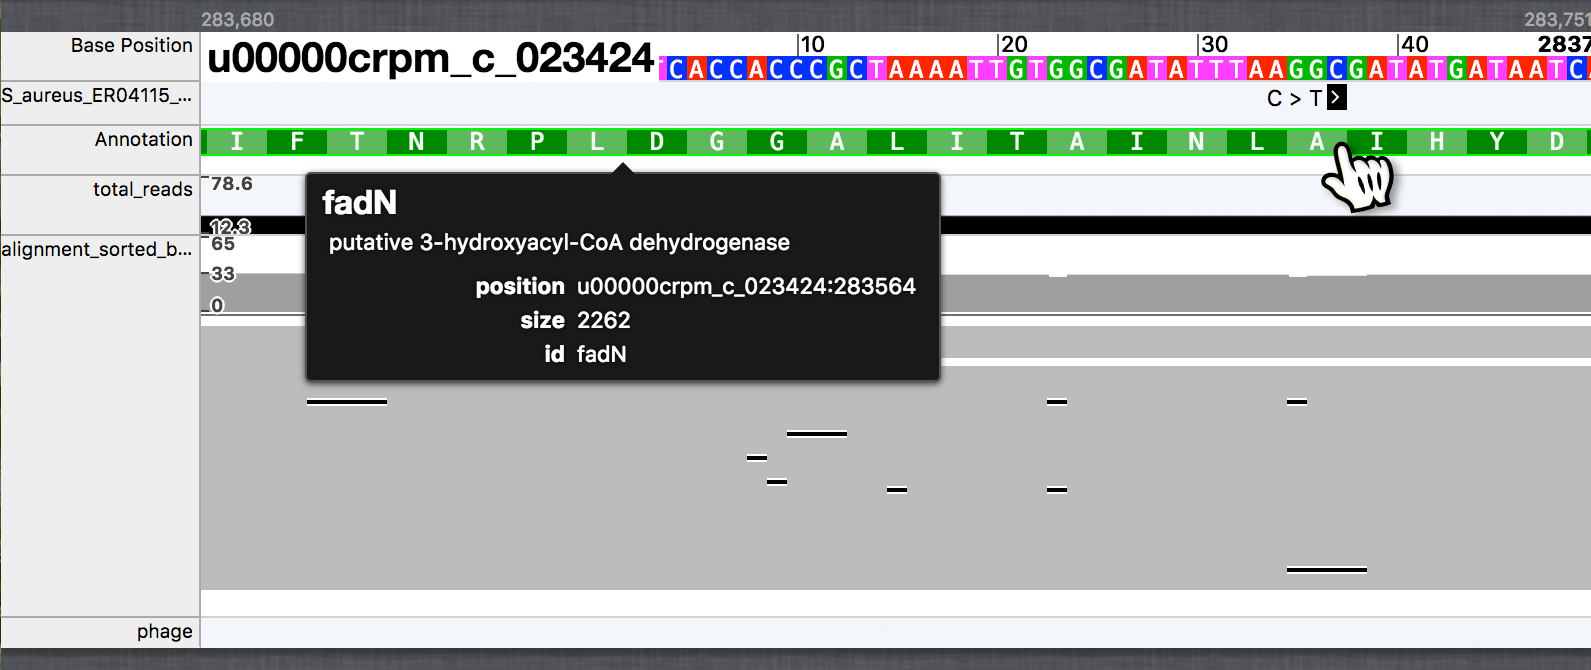
\includegraphics[width=\textwidth]{chap3/bacterial-snv}               
  \caption[A SNV between the two \emph{S. aureus} strains is in \emph{fadN}]{A SNV between the two \emph{S. aureus} strains is in \emph{fadN}, which putatively encodes a 3-hydroxyacyl-CoA dehydrogenase. Note that \emph{fadN} is on the negative strand while the SNV annotation (top track) is relative to the positive strand.}
  \label{fig:bacterial_phage_variability}
\end{figure*}
The surrounding region appears to have good, even coverage of the error-corrected reads and generally good alignment between those reads.\footnote[][1cm]{After error correction of PacBio RSII reads, the most typical remaining errors are short indels, as seen above.} Therefore, this variant call likely reflects a real SNV, although for completeness, the locus for the corresponding SNV in the reverse comparison should also be examined. It is in a \emph{fadN} gene, whose homolog was previously identified in \emph{Bacillus subtilis} to be part of a 3-hydroxyacyl-CoA dehydrogenase/enoyl-CoA hydratase complex, which is involved in fatty acid degradation.\autocite{Matsuoka2007} The depicted variant, which is aligned to the positive strand while the \emph{fadN} annotation is on the reverse strand, would cause a nonsynonymous Ala-697→Thr mutation. Since both isolates were both cultured from active infections, we can glean that this mutation is not likely to be deleterious to fatty acid degradation in \emph{S. aureus}. A more detailed analysis is beyond the scope of this article. This example, however, illustrates value of ChromoZoom in quickly being able to viewing and diagnose bacterial genome assembly and variant call quality, particularly when infectious disease clinicians are expecting to use the data to provide evidence for or against transmission, with the timeliness of infection control interventions and the prevention of a potential outbreak at stake.

\subsection{Browsing NGS data for a human genome}

ChromoZoom v2 is equally adept at browsing NGS data aligned to the human (or other vertebrate) reference genome, as is increasingly common in biomedical research and clinical diagnostic testing.
\begin{figure*}[htb]
  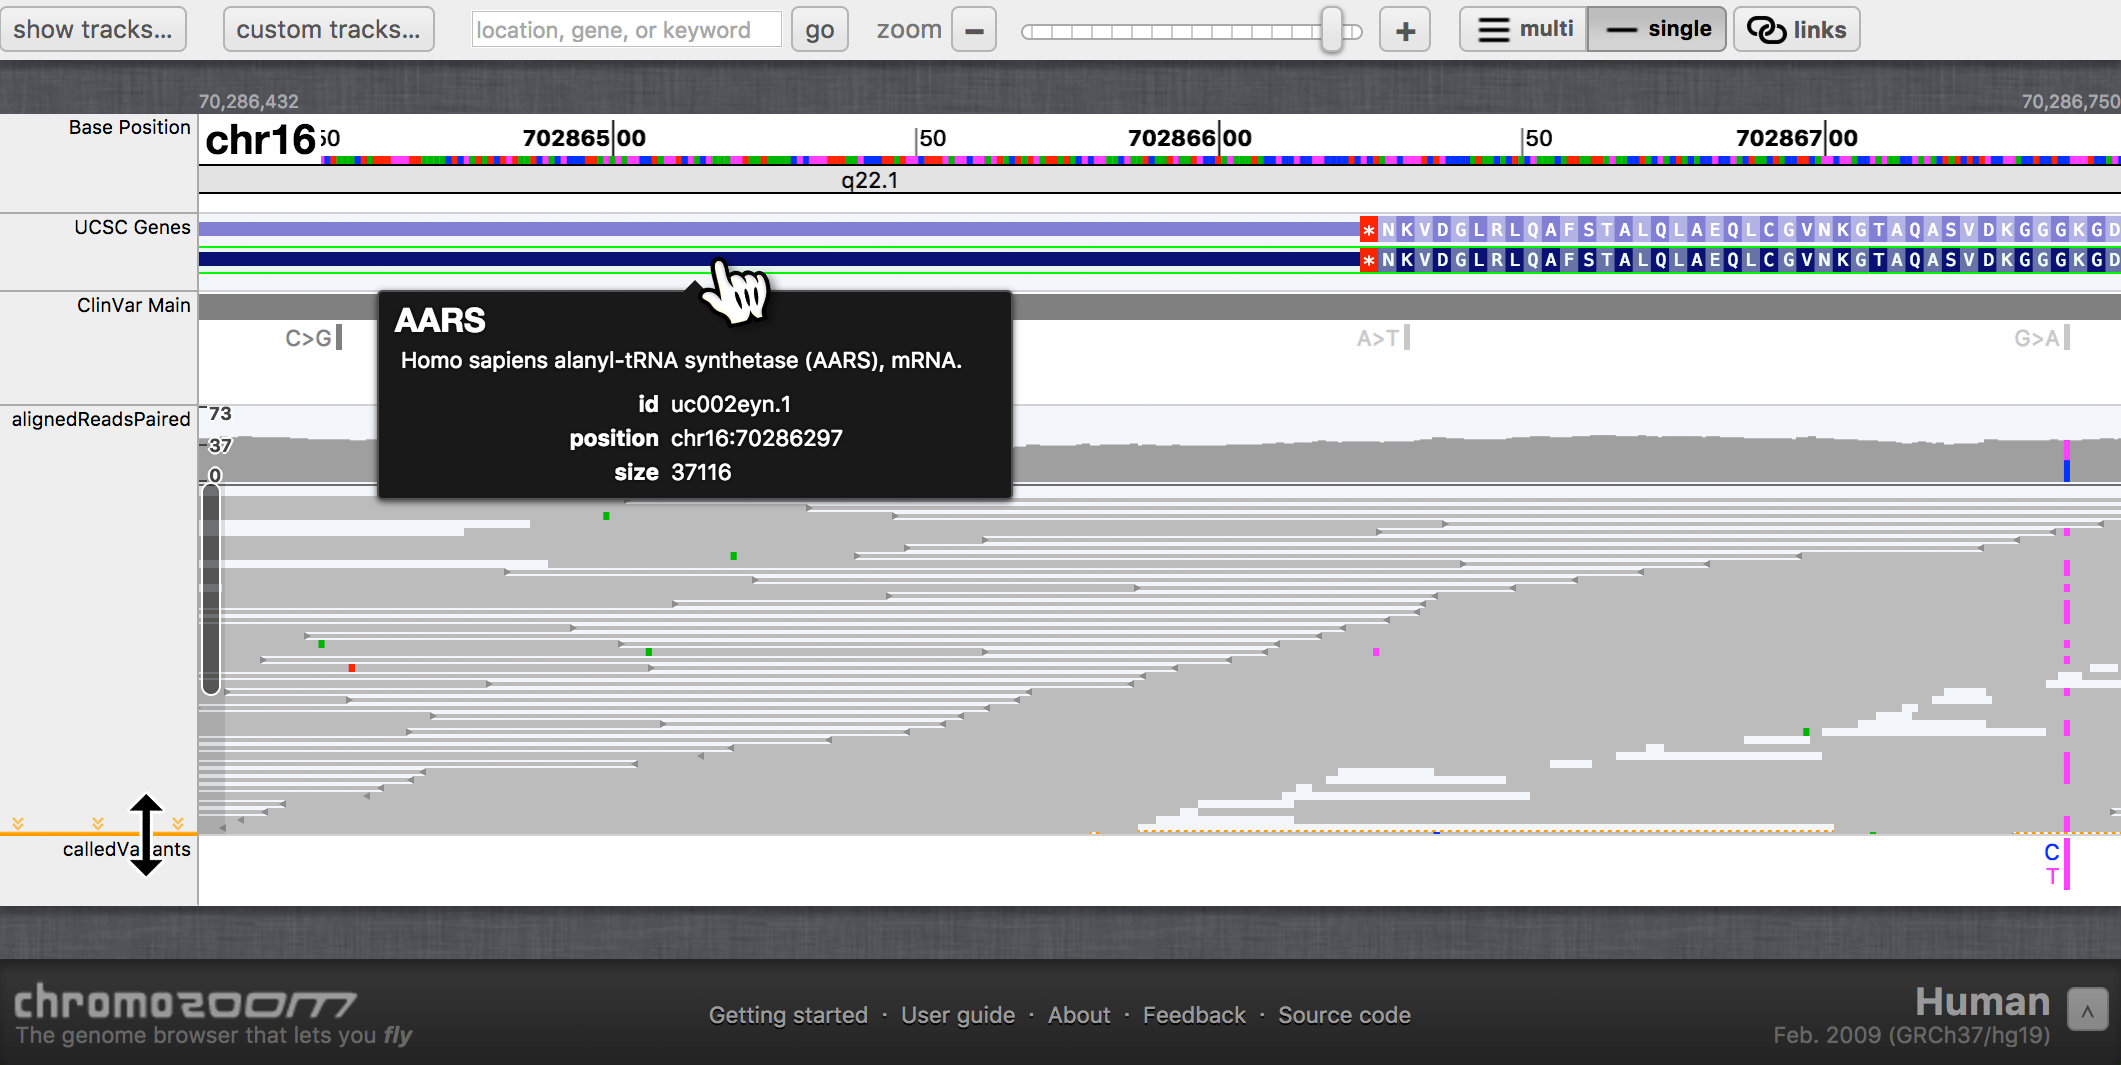
\includegraphics[width=\textwidth]{chap3/human-hg19}               
  \caption[NGS reads for the author's genome aligned to hg19]{\textbf{NGS reads for the author's genome aligned to hg19}, displayed in paired mode, and corresponding variant calls. The ``UCSC Genes'' and ``ClinVar Main'' tracks are mirrored from UCSC, while the other two are custom tracks loaded from URLs provided by the user; ``alignedReadsPaired'' is in BAM format while ``calledVariants'' is a tabix-compressed VCF file. A heterozygous C/T variant in the AARS coding sequence is visible to the righthand side, which is annotated in the ClinVar track as a benign variant (light gray G>A; annotated to reverse strand). More alignments are stacked vertically than can be displayed, as indicated by the orange clipping indicator, which could be remedied by resizing the tracks or using the adjacent scrollbar.\vspace{1em}}
  \label{fig:human-hg19}
  \setfloatalignment{b}
\end{figure*}
Figure \ref{fig:human-hg19} depicts a ChromoZoom v2 visualization of NGS reads for the author's genomic DNA generated as part of the Practical Analysis of a Personal Genome class offered at Mount Sinai.\autocite{Linderman2015} Sequencing was performed to approximately 30-fold mean coverage on an Illumina HiSeq using a 100bp paired-end protocol. As described in Implementation, for reference genomes curated by UCSC, we utilize a track scraper to pull links to all supported track types in UCSC's MySQL database (with local conversion to the bigBed format as necessary) to give ChromoZoom users instant access to 7,969 curated tracks for the hg19 reference. Clicking items in these tracks (such as the AARS gene in Figure \ref{fig:human-hg19}) takes the user to corresponding item details page in UCSC.

\begin{marginfigure}
  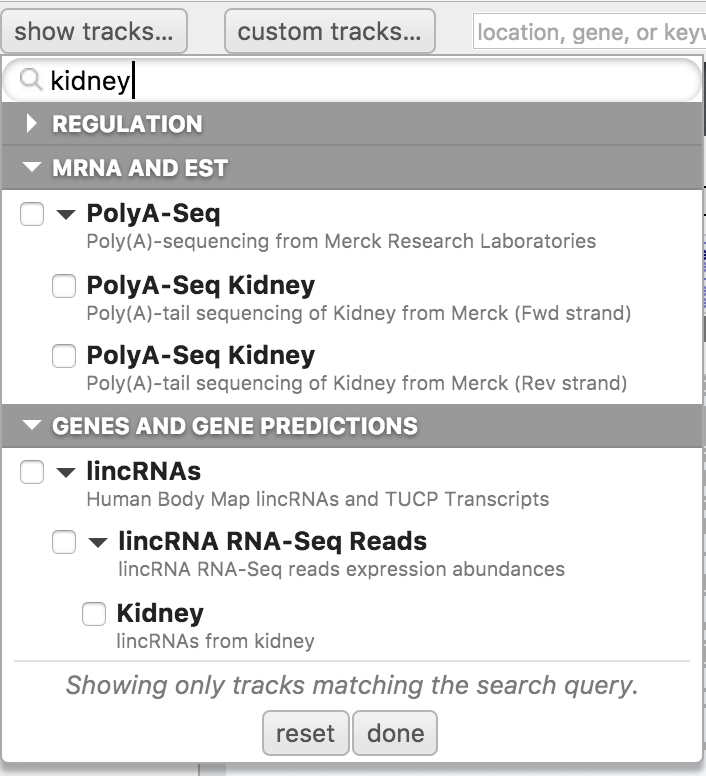
\includegraphics[width=\textwidth]{chap3/track-search}               
  \caption[Track searching interface for UCSC reference genomes.]{A searchable track interface allows quick discovery of relevant tracks from thousands of tables pulled from UCSC's databases, which can be added with a single click.}
  \label{fig:track-search}
\end{marginfigure}

With so many available tracks, navigating and selecting interesting annotations can be challenge to squeeze into the UI without creating a view that overwhelms the user. ChromoZoom v2 takes the approach of a searchable, expandable list of tracks organized in the same hierarchy used by UCSC (Figure \ref{fig:track-search}). In this UI, discoverability is still prioritized by showing an initial list of 11 collapsible categories, with only 10-20 tracks each; however, should the user be interested in a particular keyword, like ``kidney'', they can start typing it, which immediately pulls relevant tracks to the forefront of the hierarchy and filters the list to the matching subtracks. At this point, adding tracks of interest is as simple as clicking checkboxes.

\begin{marginfigure}
  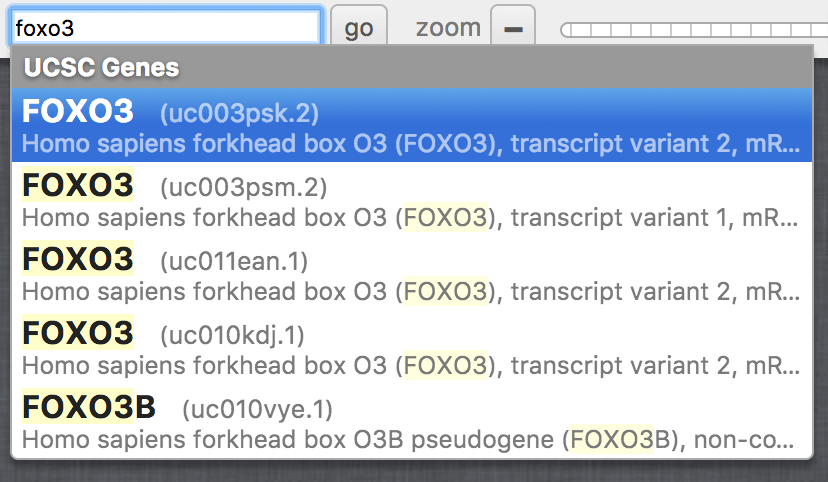
\includegraphics[width=\textwidth]{chap3/gene-search}               
  \caption[Searching for a gene by name.]{On all UCSC reference genomes, the primary gene track can be prefix-searched by name or ID, and any visible annotation tracks will also be prefix-searched (e.g., if the Human mRNAs track is open, GenBank accessions for this track will be included in the search).}
  \label{fig:gene-search}
\end{marginfigure}

Searchable indexes are seen in Figure \ref{fig:gene-search}. Lorem ipsum dolor sit amet. Ut quis urna interdum tortor sollicitudin iaculis. Aliquam purus est, venenatis ac blandit quis, semper quis felis. Integer arcu augue, accumsan at vulputate sed, tristique eu libero. Vivamus ut scelerisque massa. Pellentesque commodo arcu mollis dolor venenatis eleifend. 

\begin{figure*}[tbp]
  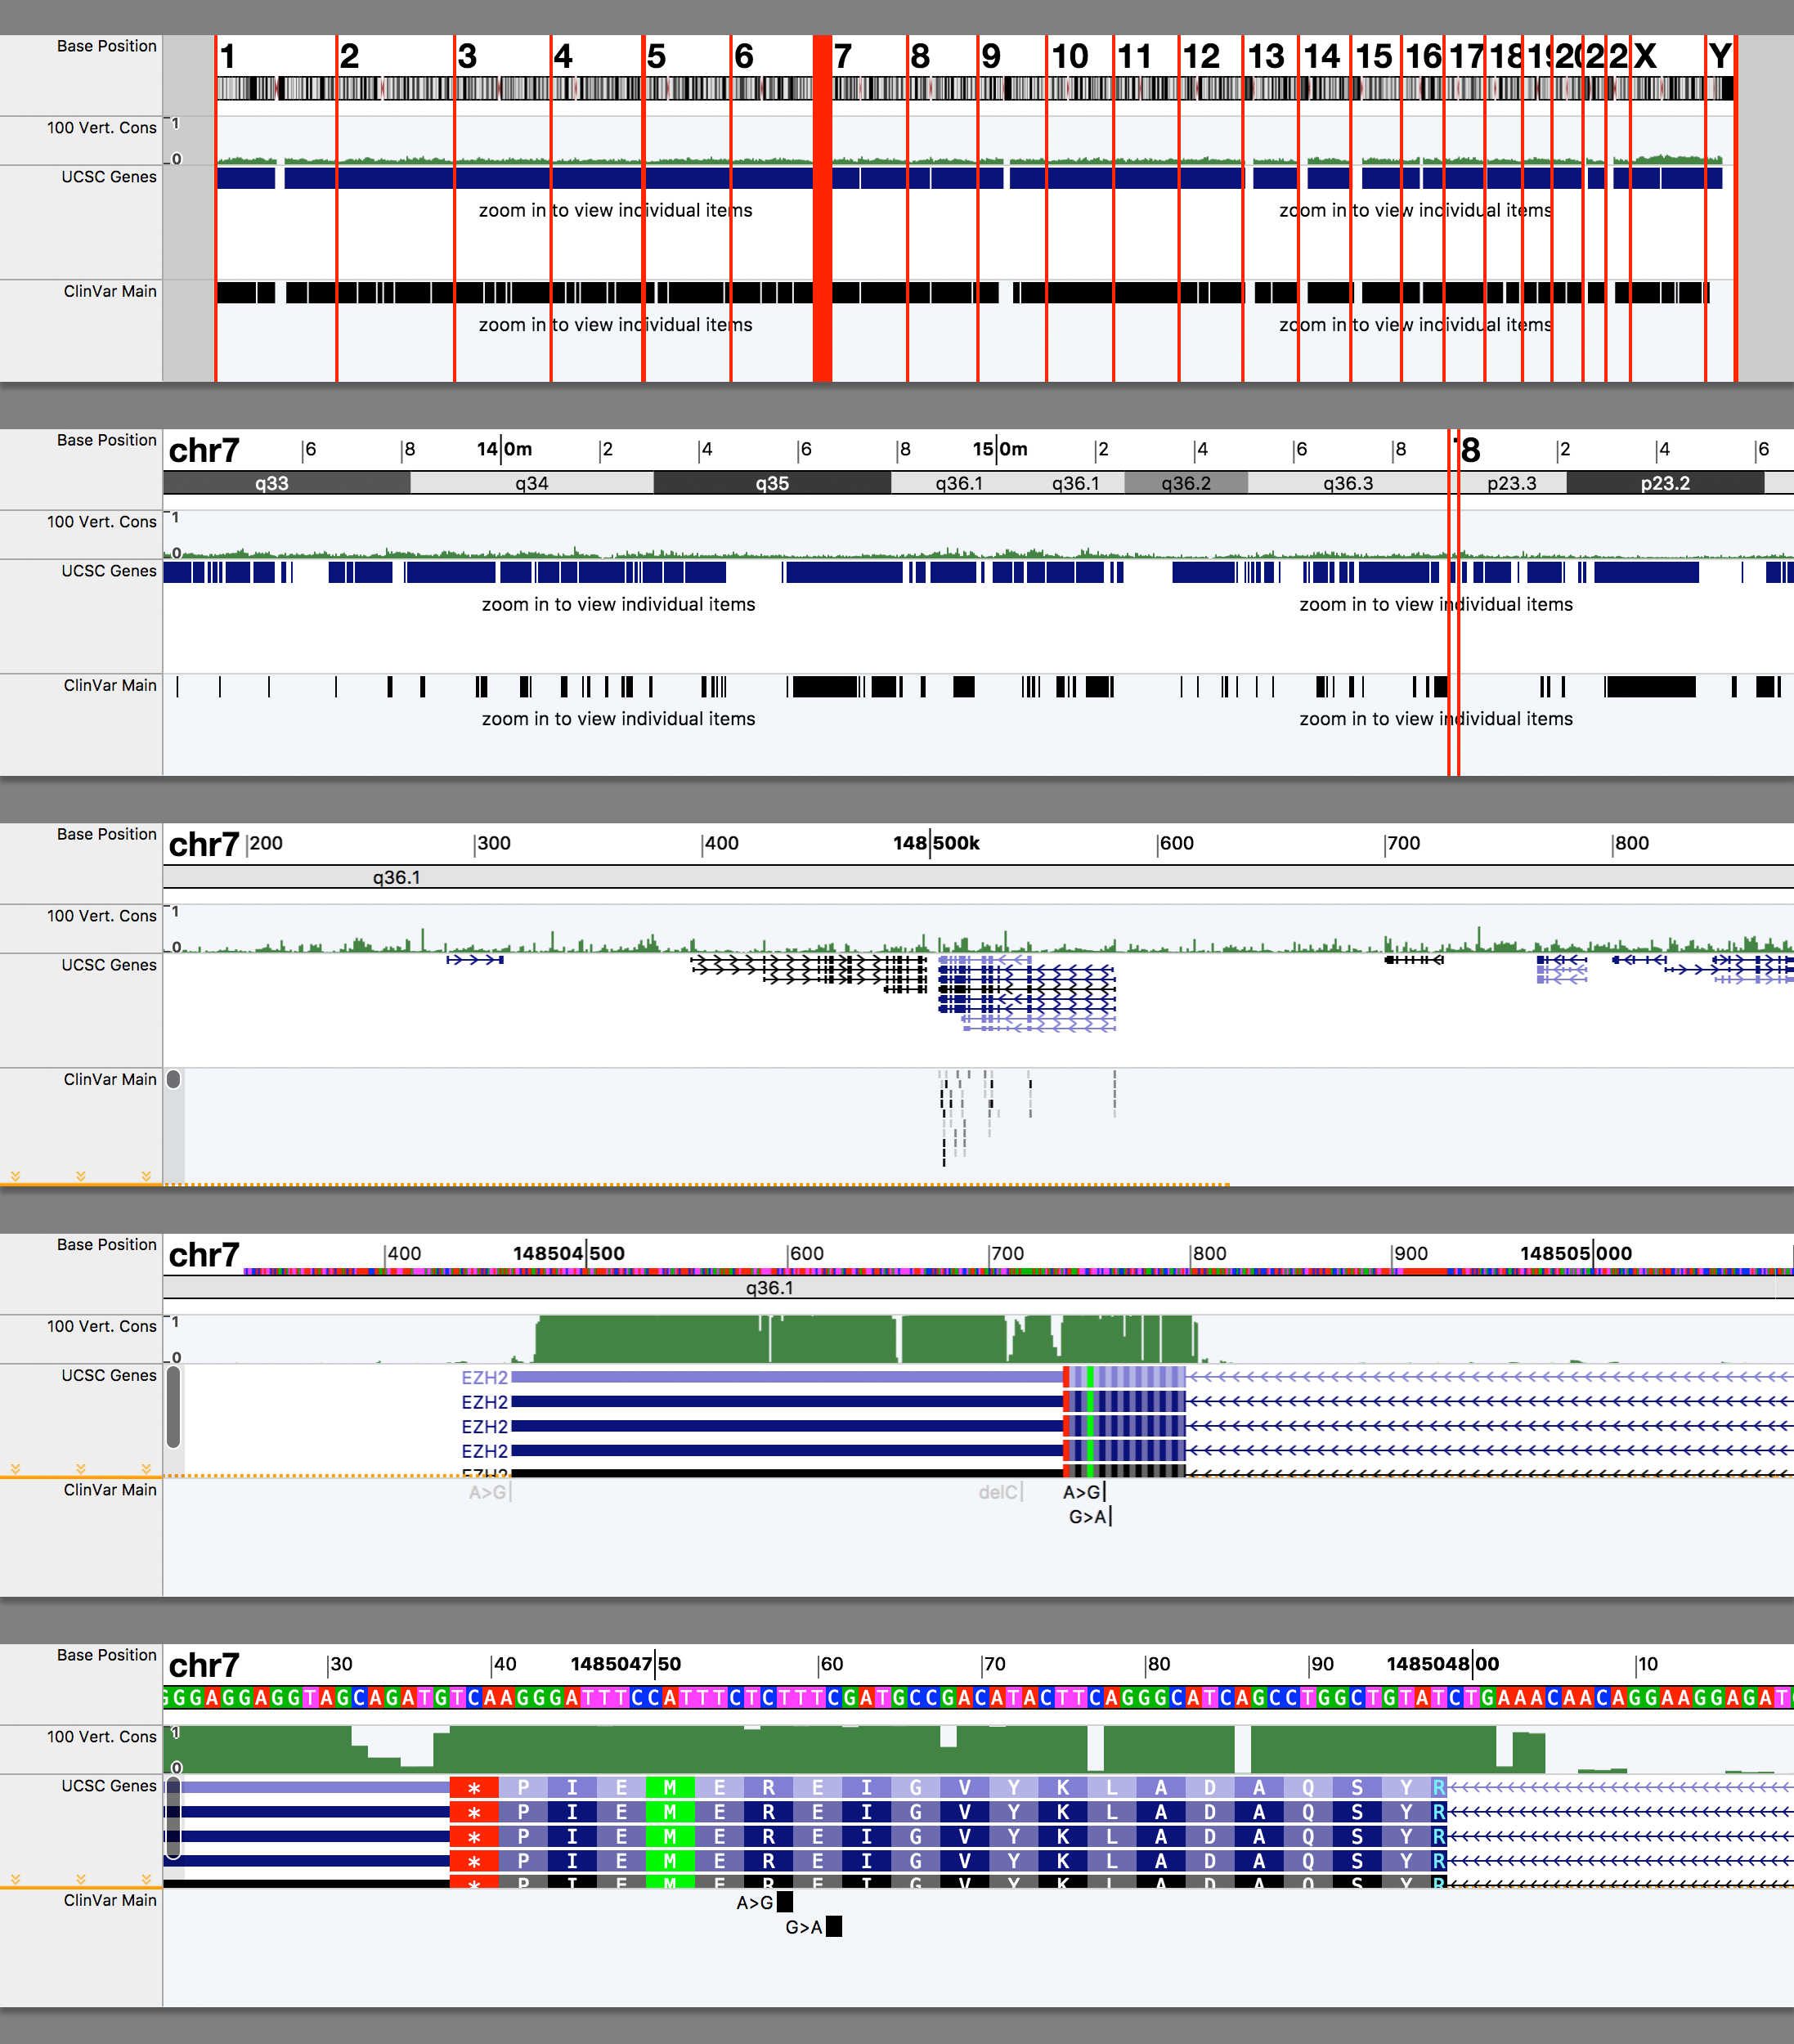
\includegraphics[width=\textwidth]{chap3/human-hg19-weaver}               
  \fullwidthlabelcaption{fig:human-hg19-weaver}{ChromoZoom dynamically redraws ticks and tracks}{
    \textbf{ChromoZoom dynamically redraws ticks, ideograms, and tracks to suit the user's current track heights and zoom level.} The above shows a series of progressive zoom operations on three UCSC-curated tracks for the hg19 reference genome, starting from a view of all chromosomes and contigs and moving in towards a view of two specific variants within the \emph{EZH2} gene. The top track displays base position and ideogram bands, which are automatically redrawn as nucleotide data as the zoom level increases. A bigWig track displaying conservation of the sequence across 100 vertebrates is immediately underneath, followed by UCSC's gene track and the same ClinVar track pictured in \ref{fig:human-hg19}. The only interaction required to move from the top view to the bottom view is a rotation of the mousewheel while pointing at the region of interest.
  }
\end{figure*}

We are really good at adapting the display to the user's zoom level. See Figure \ref{fig:human-hg19-weaver}.

\subsection{Supported genome formats}

Lorem ipsum.

\subsection{Supported track formats}

Lorem ipsum.

\subsection{Conclusions}

Lorem ipsum.

\section*{Notes}

\subsection{Contributions}

Theodore Pak wrote the first and second versions of ChromoZoom. Miha Skalic and Adrian Pasculescu contributed to the Python pipeline for mirroring data from UCSC Genome Browser. Frederick ``Fritz'' Roth provided advice and support during the initial development of ChromoZoom and throughout the development of the second version.

\subsection{Funding}

Funding was provided by the Icahn Institute for Genomics and Multiscale Biology at Mount Sinai and NIH/NIAID (U19-AI118610 and F30-AI122673).

\subsection{Conflict of Interest}

The authors have no conflicts of interest to disclose.

\subsection{Acknowledgements}

We thank Andrew Kasarskis and Miguel Ranjo for their contributions. This work was supported in part by the resources and expertise of the Department of Scientific Computing at the Icahn School of Medicine at Mount Sinai.
